\documentclass{article}
\usepackage{listings}
\usepackage{graphicx}
\begin{document}

%=================================================================================

\title{Implementation of I2C Slave in Scenario-Aware Data Flow Model of Computation using ForSyDe}
\author{Tiago Pereira Vidigal}
\maketitle

%=================================================================================

\section{Introduction} \label{sec:intro}
% Talk about SADF
% Talk about ForSyDe
% Talk about I2C
% Objective is to implement I2C Slave module using MoC SADF in ForSyDe

%=================================================================================

\section{I2C Bus and Protocol} \label{sec:proto}
% resume the "1. Introduction" section of standard
%=========================
\subsection{Specification}
%=========================
\subsection{Protocol}
%=========================
\subsection{Mandatory Features}

%=================================================================================

\section{I2C Slave} \label{sec:slave}
% I2C Slave, only mandatory features
The case of study in this project is an I2C slave module. For simplicity, only the mandatory features are implemented. It's responsible of converting user requests into the equivalent I2C stimulus. As a standard, user signals are orange, while I2C signals are grey.

% show image of pinout
\begin{figure}
  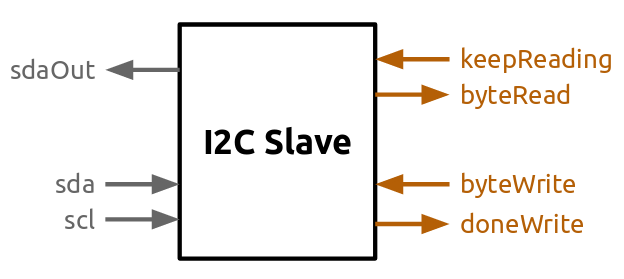
\includegraphics[width=\linewidth]{img/pinout.png}
  \caption{Pinout of the module}
  \label{fig:pinout}
\end{figure}

% Brief about parts (basic signals, address, operations)
It's implementation is divided in 3 parts: basic signals, address monitor and operations. The basic signals are a group of processes responsible for generating basic control tokens, like START and STOP conditions, as well as positive and negative edge of SCL. Address monitor is responsible of getting the address sent by the Master and checking if it matches the slave's address. Operations is the biggest part and takes care of all read and write features.

% show image of overview
\begin{figure}
  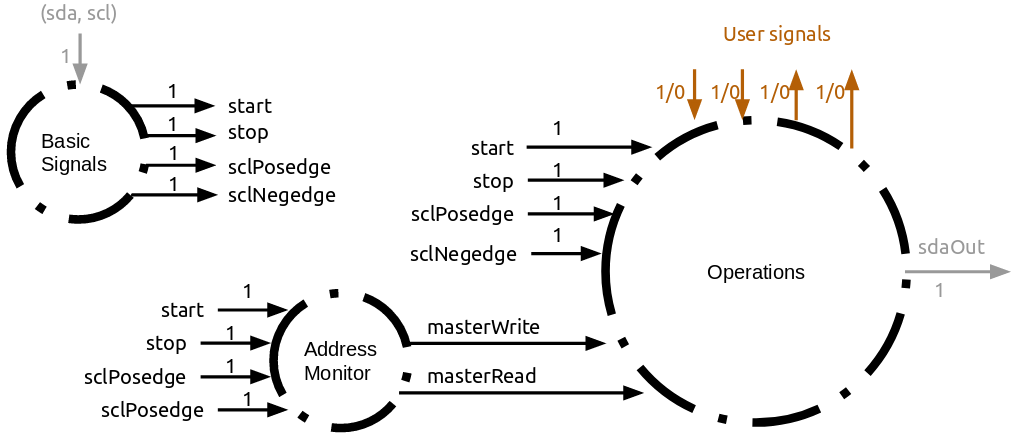
\includegraphics[width=\linewidth]{img/overview.png}
  \caption{Overview of the system. The customized circles represent groups of SADF processes}
  \label{fig:overview}
\end{figure}

% START/STOP conditions can occur at any time
% Because of that, we can't accumulate tokens
% requires to consume tokens every iteration
The I2C protocol defines a synchronous communication. However, START and STOP conditions are assynchronous and can happen at any time. An oversampling of the transmission lines is required and every value must be analyzed. This causes that processes always consume one token of I2C and basic signals, so they can keep up with unexpected conditions. Accumulation of those tokens was considered impossible for the implementation.

%=========================
\subsection{Basic signals}
Basic signals are auxiliary control tokens that give informations of the current (SDA,SCL) tuple. Their objective is to simplify the other processes. They are simple kernels with a single scenario, but with a feedback with the previous tuple.
\begin{figure}
  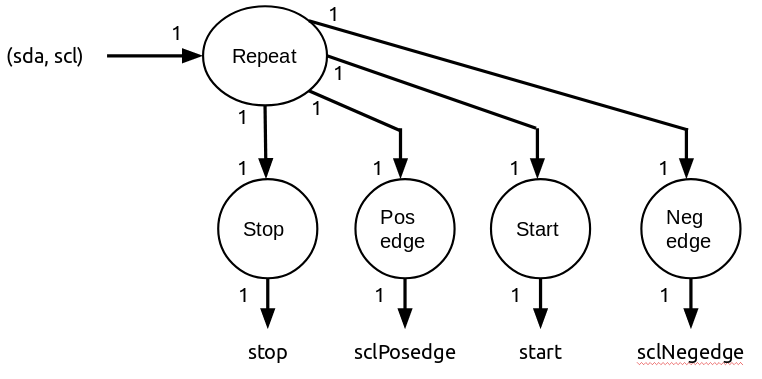
\includegraphics[width=\linewidth]{img/block_basic.png}
  \caption{Basic signals in SADF}
  \label{fig:block_basic}
\end{figure}

%=========================
\subsection{Address Monitor}
Address monitor will wait until a START condition occur. In this case, it records the next 7 received bits and check if it's equal to the slave's address. If matches, the next bit is defines which operation will be performed: Master Read or Master Write.
\begin{figure}
  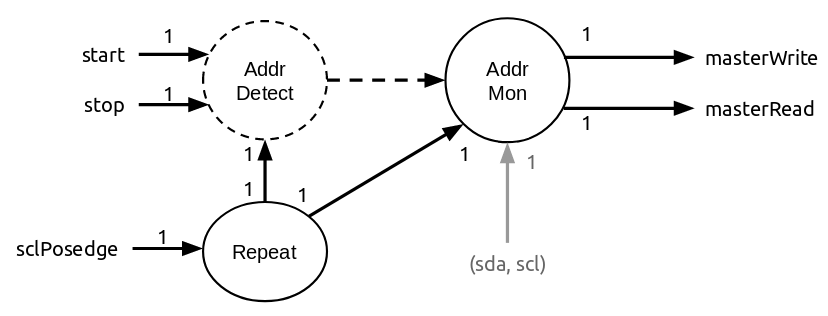
\includegraphics[width=\linewidth]{img/block_address.png}
  \caption{Address Monitor in SADF}
  \label{fig:block_address}
\end{figure}

%=========================
\subsection{Operations}
The operations are implemented with 3 detectors and 3 kernels. The detectors were merged in the Control process and it defines the scenario of each kernel. The kernels receive or send bytes according to the operation defined by the Address Monitor process.
\begin{figure}
  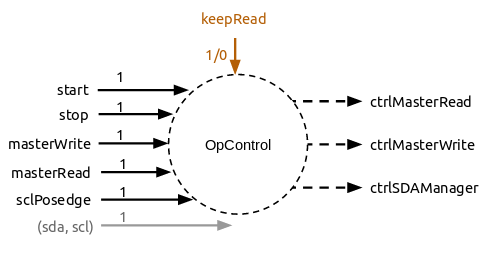
\includegraphics[width=\linewidth]{img/block_control.png}
  \caption{Operations Control detector in SADF}
  \label{fig:block_control}
\end{figure}

The operations are implemented by the respective blocks. They should never operate at the same time and they send tokens only to the SDA Manager. The manager is responsible for defining the output value in the negative edge of the SCL. On these blocks, user signals are used to define how the slave should behave during the transmission.
\begin{figure}
  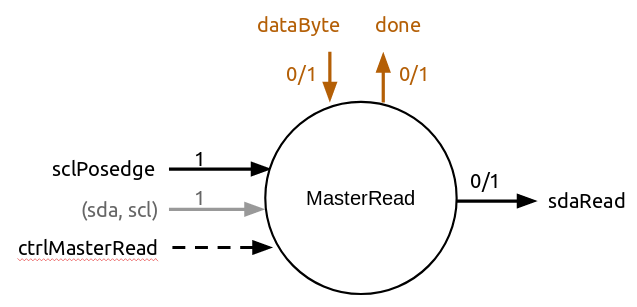
\includegraphics[width=\linewidth]{img/block_read.png}
  \caption{Operation Master Read kernel in SADF}
  \label{fig:block_read}
\end{figure}
\begin{figure}
  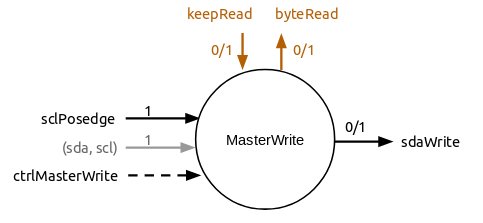
\includegraphics[width=\linewidth]{img/block_write.png}
  \caption{Operation Master Write kernel in SADF}
  \label{fig:block_write}
\end{figure}
\begin{figure}
  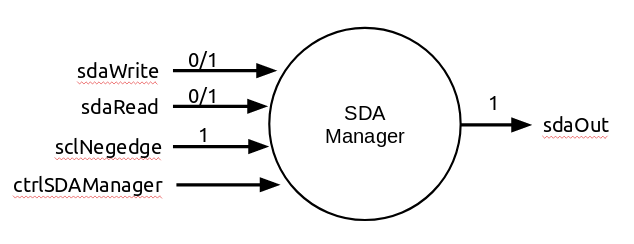
\includegraphics[width=\linewidth]{img/block_sda.png}
  \caption{Operation SDA Manager kernel in SADF}
  \label{fig:block_sda}
\end{figure}

%=================================================================================

\section{Implementation} \label{sec:imple}
The implementation was divided in multiple files. Each process contains it's own file to improve manutenability. The following tree was generated according to what was discussed in Section \ref{sec:slave}.
\begin{lstlisting}[frame=single, basicstyle=\small, caption={Files of implementation}, captionpos=b]
src
|-- I2CSlaveAddressMonitor.hs
|-- I2CSlaveGlobals.hs
|-- I2CSlave.hs
|-- I2CSlaveNegedge.hs
|-- I2CSlaveOpControl.hs
|-- I2CSlaveOpRead.hs
|-- I2CSlaveOpWrite.hs
|-- I2CSlavePosedge.hs
|-- I2CSlaveSDAManager.hs
|-- I2CSlaveStart.hs
|-- I2CSlaveStop.hs
'-- SADF.hs
\end{lstlisting}
Many of those processes are currently under development. The focus of this report will be the I2CSlaveStart kernel. The auxiliary file I2CSlaveGlobals is used by all the files, so will be described as well.

%=========================
\subsection{I2CSlaveGlobals}

The I2CSlaveGlobals is a unified source for all the types and constants used throughout the system. At ForSyDe, no classes were defined to model the inputs for SADF MoC. Aliases were created to bypass this lack, improving readability and manutenability of the program.
\begin{lstlisting}[frame=single, basicstyle=\small, language={Haskell}, caption={Alias for the Condition's scenario type}, captionpos=b]
-- | Scenario (rates) for a condition kernel
--
-- inRates = Consumption rates
--    1: SDA and SCL lines current value
--    2: SDA and SCL lines past value
-- outRates = Production rates
--    1: condition occurred (or not)
-- execFunc = Function that models operation
--    Arg 1:  current values token
--    Arg 2:  past values token
--    Return: condition token
type ScenarCondition = ((Int,Int),
                        Int,
                        [(Int,Int)] -> [(Int,Int)] -> [Int])
\end{lstlisting}

%=========================
\subsection{I2CSlaveStart}

The I2CSlaveStart is a kernel responsible for detecting START conditions. This is done by checking both current and past values of the I2C bus. A feedback provides the previous values, while the current comes directly from the input.
A START condition happens when both SDA and SCL were high and then only SDA drops. In this case, the output token will be generated with the value '1'. Otherwise, the token will contain the value '0'.
\begin{lstlisting}[frame=single, basicstyle=\small, language={Haskell}, caption={START condition detector in Haskell}, captionpos=b, label={lst:behaviour}]
conditStart :: [(Int,Int)]
            -> [(Int,Int)]
            -> [Int]
conditStart [] _   = []
conditStart inputs pastInputs = map checkStart inputSequence
  where inputSequence = (zip pastInputs inputs)
        checkStart (past, current)
          | past     /= (1,1) = 0
          | current  == (0,1) = 1
          | otherwise         = 0
\end{lstlisting}

Once it's a simple process, a single function and scenario are required for it's operation. That way, the only scenario in which the kernel will operate is 'startScenar'.
\begin{lstlisting}[frame=single, basicstyle=\small, language={Haskell}, caption={Unique START condition scenario}, captionpos=b]
-- | START scenario
startScenar :: ScenarCondition
startScenar = ((1,1), 1, conditStart)
\end{lstlisting}

We could leave the kernel without a control port, as pointed in \{REFERENCE TO A Scenario-Aware Data Flow for Combined...\}. The SADF library don't have such implementation, so a list of 'startScenar' is used instead of a detector process. This approach simplifies the process and improves readability.
\begin{lstlisting}[frame=single, basicstyle=\small, language={Haskell}, caption={START condition kernel with constant scenario}, captionpos=b]
kernelStart :: Signal (Int,Int)
            -> Signal Int
kernelStart inputs = start
  where start      = kernel21SADF control inputs pastInputs
        control    = signal (repeat startScenar)
        pastInputs = delaySADF [(1,1)] inputs
\end{lstlisting}

%=========================
\subsection{I2CSlaveStart\_tb}

To validate the I2CStart kernel, a simple testbench was developed. Two lists describe the oversampled values of both lines: SDA and SCL. The testbench prepares it to act as the input of 'conditStart' function (see listing \ref{lst:behaviour}).
The correctness is shown via terminal. Expected values list is obtained directly with 'conditStart'. Result values list is obtained with 'kernelStart'. Those are compared and the success or failure is printed. Diff list indicates mismatches.

\begin{lstlisting}[frame=single, basicstyle=\small, caption={I2CSlaveStart\_tb failure screen example}, captionpos=b]
SDA:      """\___/"""""""\_________/"""""\_______________/"""
SCL:      """""\_/"\_/"\_____/"\_/"""\_/"""\_/"\_/"\_/"""""""

Expected: [0,1,0,0,0,0,0,0,0,0,0,0,0,0,0,1,0,0,0,0,0,0,0,0,0]
Result:   [0,1,0,0,0,0,0,0,0,1,0,1,0,0,0,1,0,1,0,1,0,1,1,0,0]
Diff:     ___________________|___|___________|___|___|_|_____

####### FAILED #######
\end{lstlisting}

Testbenches are executed at the 'tb' directory. The most direct way to run is using 'runhaskell' and selecting the desired testbench. It's necessary to include the source directory for the compilation.

\begin{lstlisting}[frame=single, basicstyle=\small, caption={How to run testbench}, captionpos=b]
cd tb
runhaskell -i../src I2CSlaveStart_tb.hs
\end{lstlisting}

%=================================================================================

\section{Results} \label{sec:resul}
% still implementing, but have some partial results
The I2C Slave complete implementation is still pending. However, partial results with the 'I2CSlaveStart' kernel helped to plan an organized structure for implementation of the rest of the system. 

% I2CSlaveStart completely validated
The alias approach reduced the verbosity required by the SADF library. A separated file for the process is a good approach to simplify search and improve organization when multiple processes are required.
The developed testbench tries all combinations of the pair current and past values of the lines. The Start condition kernel is fully validated once all results matched the expected values. All basic signal processes can be implemented with very little adaptation from it.

%=================================================================================

\section{Conclusion} \label{sec:concl}
% SADF not an interesting MoC for I2C due unexpected START/STOP conditions
The SADF MoC is not very interesting to implement I2C. That's because Start and Stop conditions can occur at any time. This specification requires that all blocks monitor the basic signals on every iteration. Token accumulation will cause desynchronization, so all tokens must be consumed immediately.

% SDF/SADF libraries have not an optimal implementation
% the use of tuples obligates the implementation the way it is
% ref: https://jayconrod.com/posts/14/currying-and-why-we-don-t-pass-arguments-as-tuples
% a class approach would bring many benefits


% kernel using feedback generates an implicit state... is this valid in SADF?
The implementation created a feedback at the kernel, so past input values would be available for the next iteration. This generates an implicit state at the kernel and this might not follow the SADF modelling. This should be confirmed with further studies.

% Next works: complete the I2C Slave
The next step will be to fully implement the I2C Slave. Another four testbenches will be implemented, each with a different Design Under Test (DUT): all basic signals, address monitor processes, operation processes and top level. Also an alternative implementation in Chisel could bring interesting topics for comparison.


\end{document}
